% !TeX program = xelatex
% UTF-8；XeLaTeX 编译两次以更新目录和交叉引用。
% 插图全部读取 images/ 下的独立 PDF/PNG 文件；本文件不使用任何绘图环境。
\documentclass[UTF8,a4paper,zihao=5,fontset=fandol]{ctexart}
\usepackage[top=20mm,bottom=20mm,left=21mm,right=21mm]{geometry}
\usepackage{graphicx,float,caption,subcaption}
\usepackage{booktabs,tabularx,array,enumitem}
\usepackage[hidelinks,unicode]{hyperref}
\graphicspath{{images/}}
\hypersetup{pdftitle={实验二：软件设计与建模},pdfauthor={朱爽爽},pdfsubject={南京大学校园二手交易平台}}
\ctexset{
  section={number=\chinese{section},format=\Large\bfseries,beforeskip=1.3ex,afterskip=0.8ex},
  subsection={number=\arabic{subsection},format=\normalsize\bfseries,beforeskip=1.2ex,afterskip=0.6ex},
  subsubsection={format=\normalsize\bfseries,beforeskip=0.8ex,afterskip=0.4ex}
}
\setlength{\parindent}{2em}
\setlength{\parskip}{2pt}
\linespread{1.25}
\setlist{nosep,leftmargin=2em,topsep=3pt}
\captionsetup{font=small,skip=4pt}
\captionsetup[subfigure]{font=small,justification=centering}
\setlength{\intextsep}{7pt}
\setlength{\textfloatsep}{8pt}
\renewcommand{\arraystretch}{1.2}
\setcounter{tocdepth}{2}
\counterwithin{figure}{section}
\renewcommand{\thefigure}{\arabic{section}.\arabic{figure}}
\pagestyle{plain}
\raggedbottom
\emergencystretch=1em

% 固定图稿位置，防止图片跑到上一节或下一节。
% 参数：图片、最大高度、图题、交叉引用标记。
\newcommand{\reportfigure}[4]{%
  \begin{figure}[H]\centering
    \includegraphics[width=0.98\linewidth,height=#2,keepaspectratio]{#1}
    \caption{#3}\label{#4}
  \end{figure}}

\begin{document}

\begin{center}
  {\LARGE 软件工程\par}
  \vspace{5mm}
  {\large 实验二：软件设计与建模\par}
  \vspace{5mm}
  {朱爽爽\quad 241840080\par}
  \vspace{3mm}
  {2026年11月13日\par}
\end{center}
\vspace{3mm}
\tableofcontents
\vfill
\begin{center}
  \small 项目：栖物——南京大学校园二手交易平台
\end{center}
\clearpage

\section{软件的主要功能}
\subsection{主要功能}
本项目延续实验1的校园二手交易需求：学生通过校园邮箱注册，发布与查找闲置物品，预约后线下面交，最后由双方确认完成。管理员负责审核商品、处理违规、管理账号、查看统计和日志。第一期不加入在线支付、物流与即时聊天。

\subsection{功能模块}
系统分为账号与身份、商品与搜索、审核与治理、预约与交易、通知、统计与日志六个模块。考虑课程规模与测试成本，本设计采用单体应用方案。具体服务划分见组件图，模块之间通过业务服务协作，不把全部逻辑写在页面中。

\section{软件架构UML图}
本次使用PlantUML绘制类图、组件图、活动图、用例图、状态图和序列图，共6种。序列图按Sequence计为一种，不将“时序图”的另一种中文译名重复计数。

\subsection{结构性图（一）：类图}
\reportfigure{u01.pdf}{120mm}{核心领域类图}{fig:class}
商品与预约分开保存：商品可以有多条历史预约，但同时只能有一条有效预约。取消后保留记录，才能解释商品为什么重新可买；双方确认后才生成唯一交易结果。

交易保留商品快照，避免后续信息变化影响历史。价格以整数分保存；图片与审核记录分别关联商品，审核还要绑定版本。这里保留了必要的数据约束，而没有将页面上的每个控件都设计成一个类。
\clearpage

\subsection{结构性图（二）：组件图}
\reportfigure{u02.pdf}{163mm}{分层组件及模块协作}{fig:component}
\textbf{逻辑关系。} 浏览器请求先经过身份与归属校验，再调用业务服务。商品下架、违规处理、账号停用和超时任务都复用预约服务；通知与审计统一处理，数据库负责持久化和约束。

\textbf{设计取舍。} 商品、预约和交易结果经常需要一起更新。课程规模下，Django单体配合SQLite更容易在一个事务内处理这些变化，也减少部署和测试成本。SQLite不能依赖\texttt{SELECT FOR UPDATE}实现行锁，因此还需要条件更新、唯一约束及后续并发测试。

\textbf{边界。} 页面不显示某个按钮，只是防止误操作；真正的权限判断必须放在服务器。定时任务也走相同的状态规则，不能另写一套“过期就恢复商品”的逻辑。
\clearpage

\subsection{行为性图（一）：活动图}
\reportfigure{u04.pdf}{193mm}{从发布到交易完成的活动图}{fig:activity}
卖家提交商品后先审核，驳回则修改重提。买家预约成功后，卖家须在24小时内接受；拒绝、取消和待确认超时都会结束预约。接受后进入面交，双方分别确认，交易才算完成。

这里需要区分两个容易混淆的动作：\textbf{接受预约表示愿意保留商品，确认完成才表示交接结束。}例如，卖家今天接受预约、双方约定明天见面，此时就把商品标成“已售出”显然过早。分开这两个动作，页面也能准确提示下一步由谁操作。
\clearpage

\subsection{行为性图（二）：用例图}
\reportfigure{u03.pdf}{192mm}{参与者与功能边界}{fig:usecase}
买家与卖家不是两套账号。同一个学生可以出售自己的物品，也可以买别人的物品，权限应根据当前资源归属判断。管理员负责治理，不代替买卖双方完成交易确认；到期调度器只关闭尚未接受且已经超时的预约。

因此，“切换买家或卖家视角”只是原型中的演示入口，不是正式系统的授权机制。这一点需要在实验3通过直接请求接口来检查，不能只看页面是否隐藏了入口。
\clearpage

\subsection{行为性图（三）：状态图}
\reportfigure{u05.pdf}{160mm}{商品生命周期}{fig:state}
\textbf{下架后是否可以重上架？}完全禁止并不实用：卖家可能只是临时不方便交易。但直接恢复“已发布”，又可能让改过内容的商品绕过审核。本次采用的方案是：主动下架后允许重新提交，仍进入“待审核”；违规下架则先由管理员解除重审限制。

\textbf{预约期间是否允许修改？}买家预约的是某个价格和描述下的商品，因此预约期间冻结重要信息。卖家仍可下架，但必须同时取消有效预约并通知买家。已下架商品不能被较晚执行的超时任务恢复为公开状态。

这两项规则是设计阶段对实验1待明确事项的补充，分别兼顾了重新交易的需要和已有预约的稳定性，没有改写原需求基线。
\clearpage

\subsection{交互性图：双方确认序列图}
\reportfigure{u08.pdf}{181mm}{双方确认与唯一交易结果}{fig:sequence}
只确认一方时，保存该方确认时间，商品仍为“已预约”。双方确认齐全后，在同一事务内完成预约、生成交易记录，并将商品改为“已售出”。任一步失败都回滚，避免出现“商品已售出，但没有交易记录”的情况。

重复点击只能返回同一结果，不能再生成一笔交易。网络超时也不等于操作失败，应先查询原请求结果。相比增加更多页面，这些状态约束更影响系统是否可靠，需要在实验3通过真实数据库与故障测试验证。
\clearpage

\section{UI界面及功能描述}
页面采用浅色底、紫色主操作和分层信息呈现，大厅、交易详情和审核页使用一致的视觉规范。以下界面使用同一套按钮、表单和状态标签；照片为商品示意。

\subsection{商品大厅与详情}
\reportfigure{ui01.png}{99mm}{商品大厅}{fig:market}
\textbf{相关模块：}商品与搜索。首页支持关键词、分类和更多条件筛选，卡片优先呈现图片、价格、新旧程度及状态。完整描述留到详情页，避免把首页变成大表格。

\reportfigure{ui02.png}{77mm}{商品详情}{fig:detail}
详情集中展示商品信息和预约入口，提前说明24小时卖家确认及线下面交规则。联系方式不直接使用公开注册邮箱，以免浏览商品就暴露个人信息。
\clearpage

\subsection{注册登录与商品发布}
\begin{figure}[H]\centering
  \begin{subfigure}[t]{0.48\linewidth}\centering
    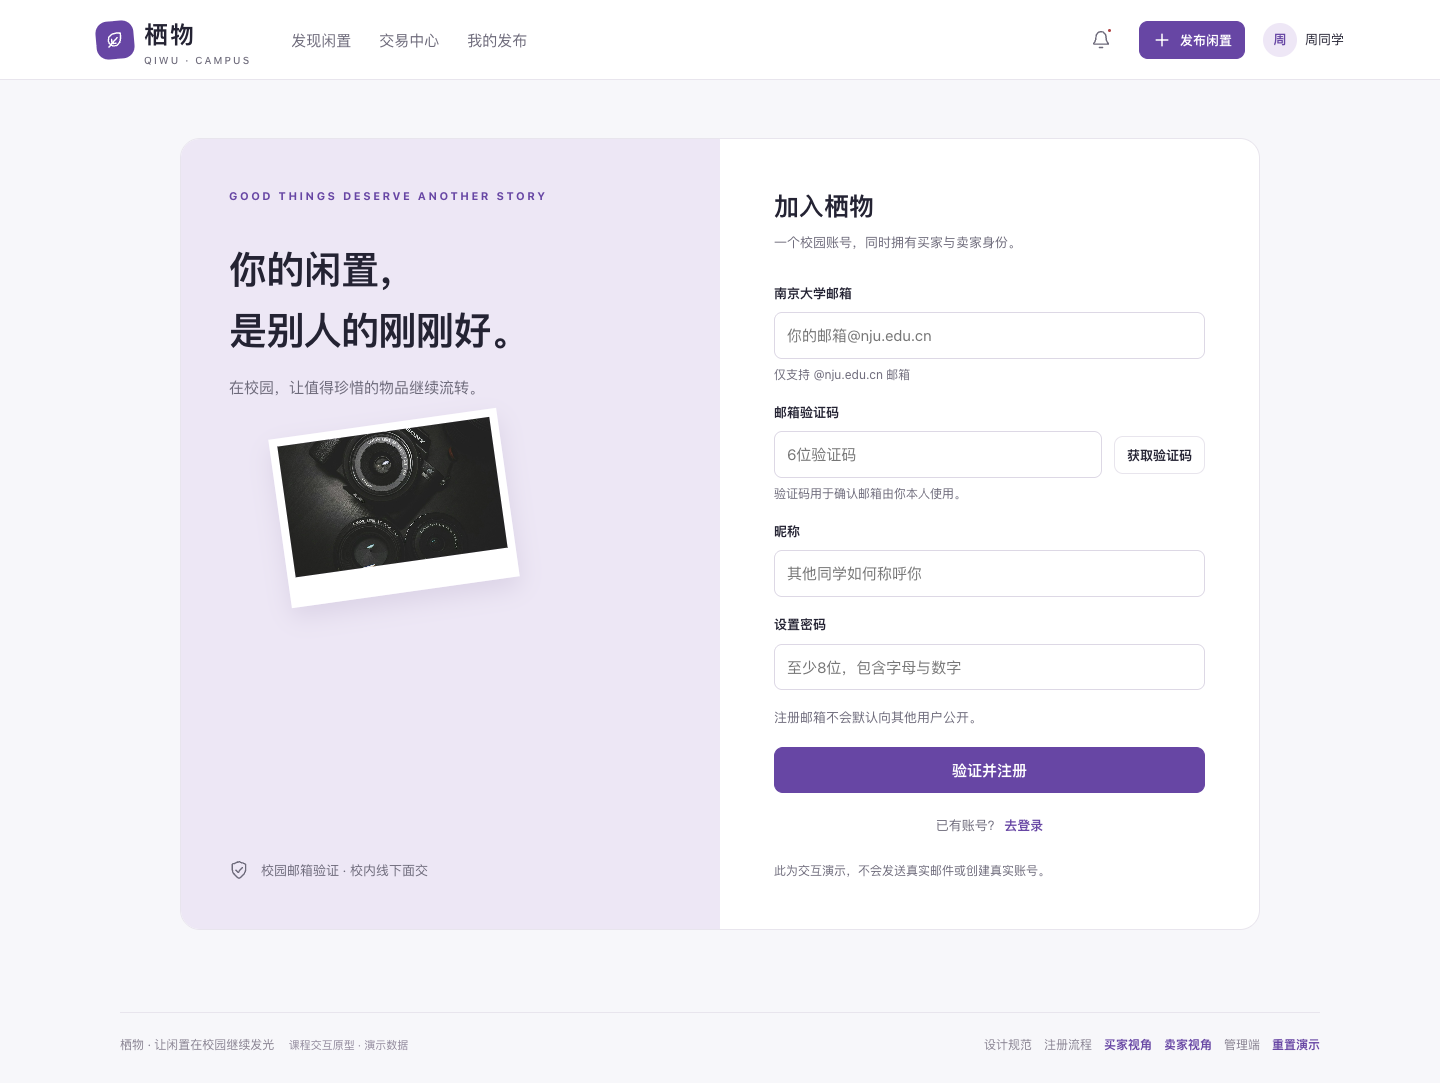
\includegraphics[width=\linewidth,height=71mm,keepaspectratio]{ui08.png}
    \caption{校园邮箱注册}
  \end{subfigure}\hfill
  \begin{subfigure}[t]{0.48\linewidth}\centering
    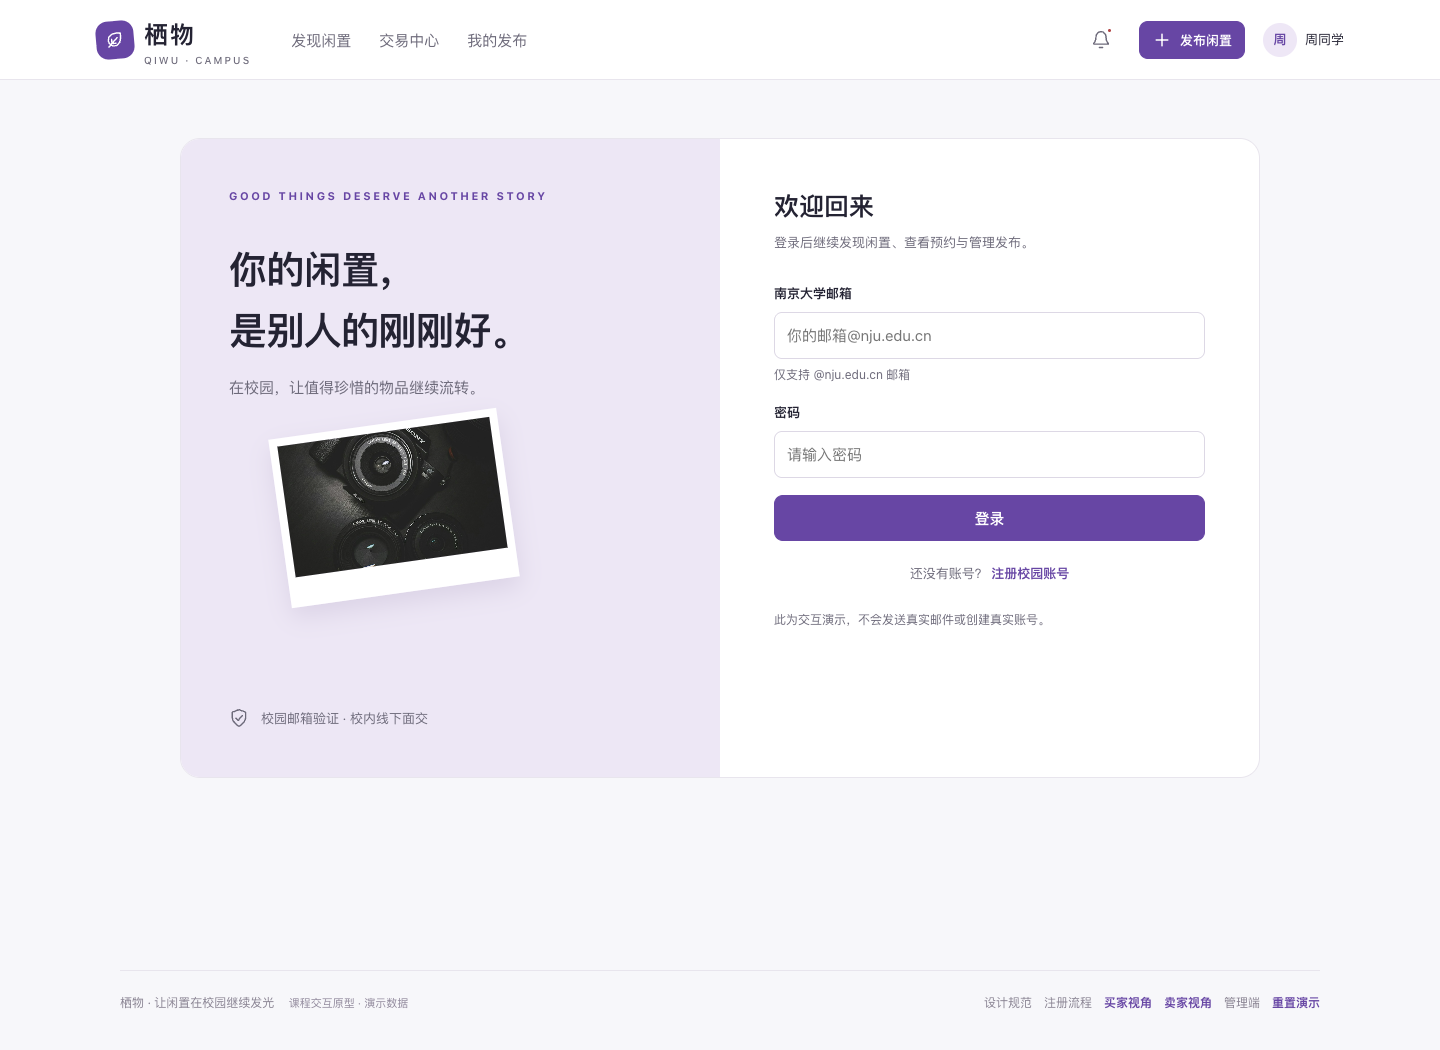
\includegraphics[width=\linewidth,height=71mm,keepaspectratio]{ui09.png}
    \caption{登录}
  \end{subfigure}
  \caption{账号入口}\label{fig:auth}
\end{figure}
\textbf{相关模块：}账号与身份。注册和登录保持单一主操作，错误说明放在输入区域附近。原型验证码仅供演示，正式实现需要邮件发送、有效期与错误次数校验。

\begin{figure}[H]\centering
  \begin{subfigure}[t]{0.48\linewidth}\centering
    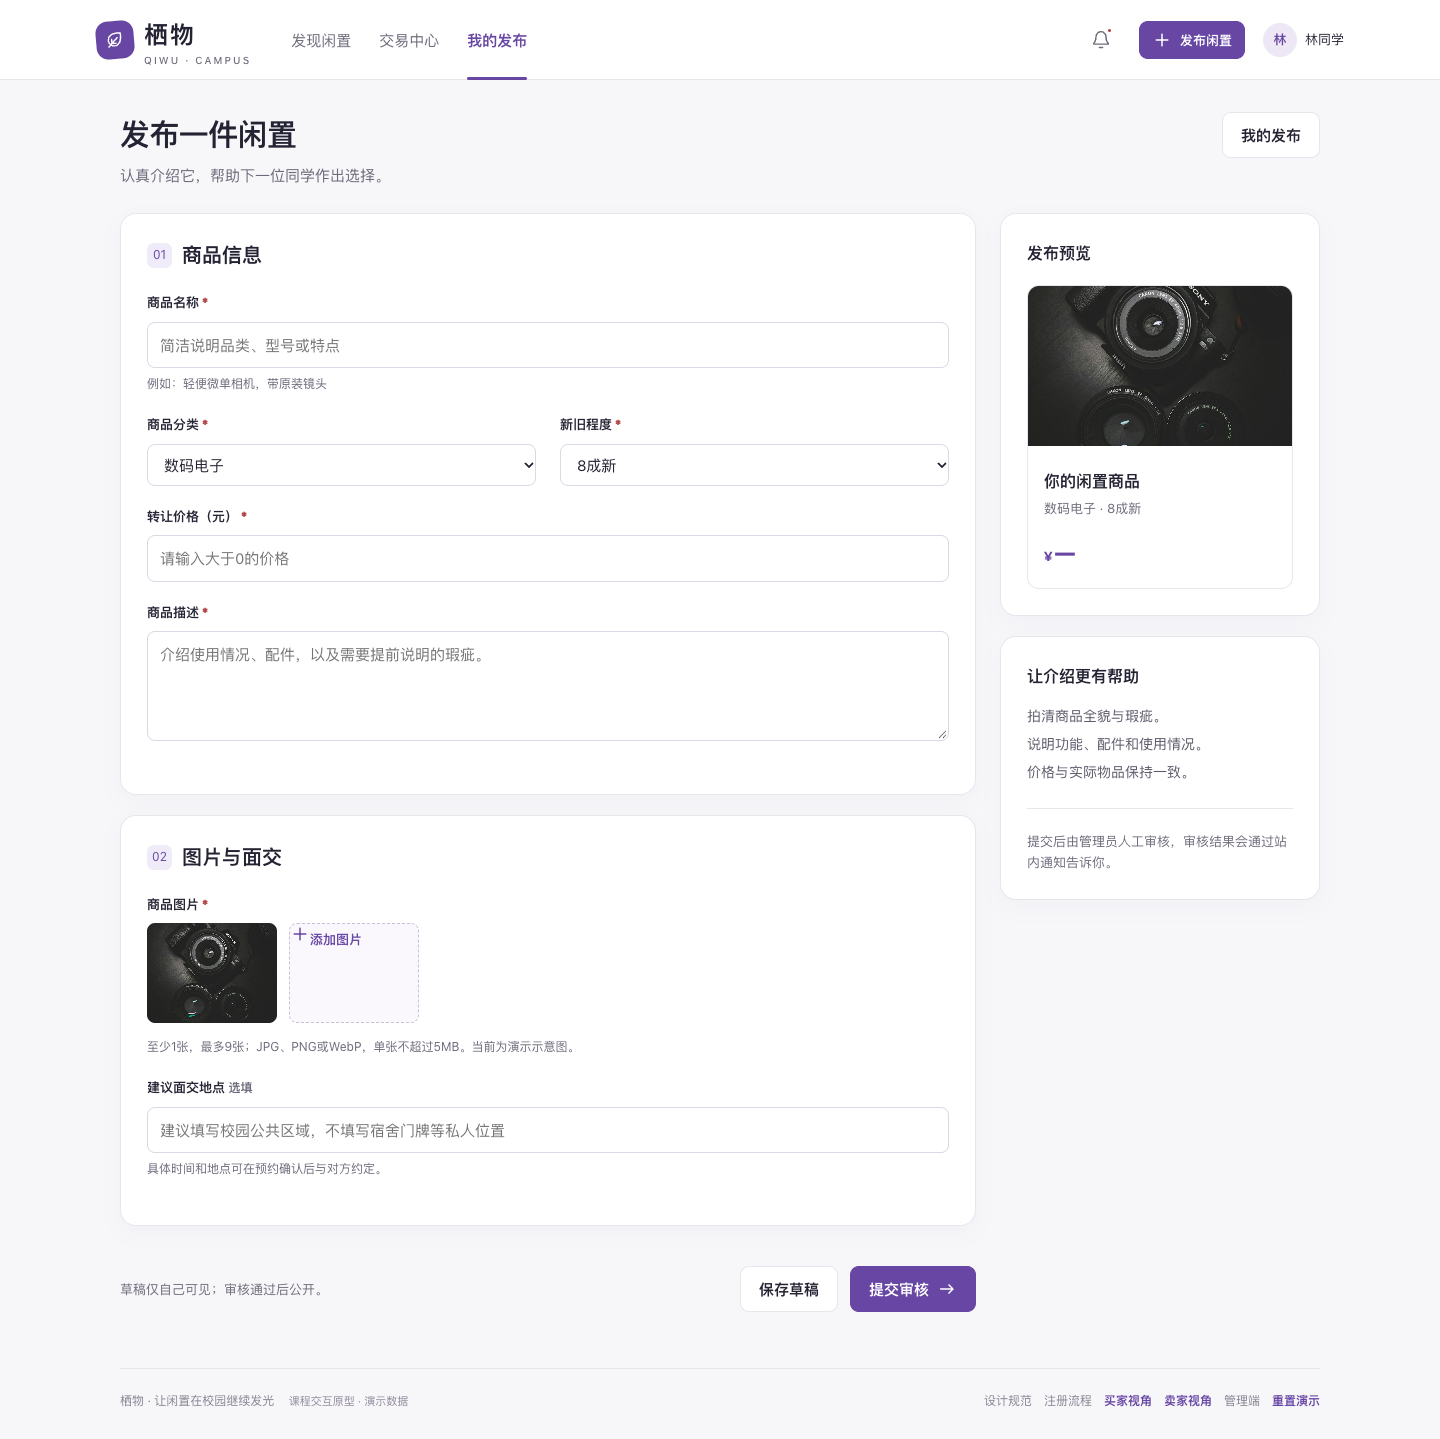
\includegraphics[width=\linewidth,height=91mm,keepaspectratio]{ui05.png}
    \caption{发布闲置}
  \end{subfigure}\hfill
  \begin{subfigure}[t]{0.48\linewidth}\centering
    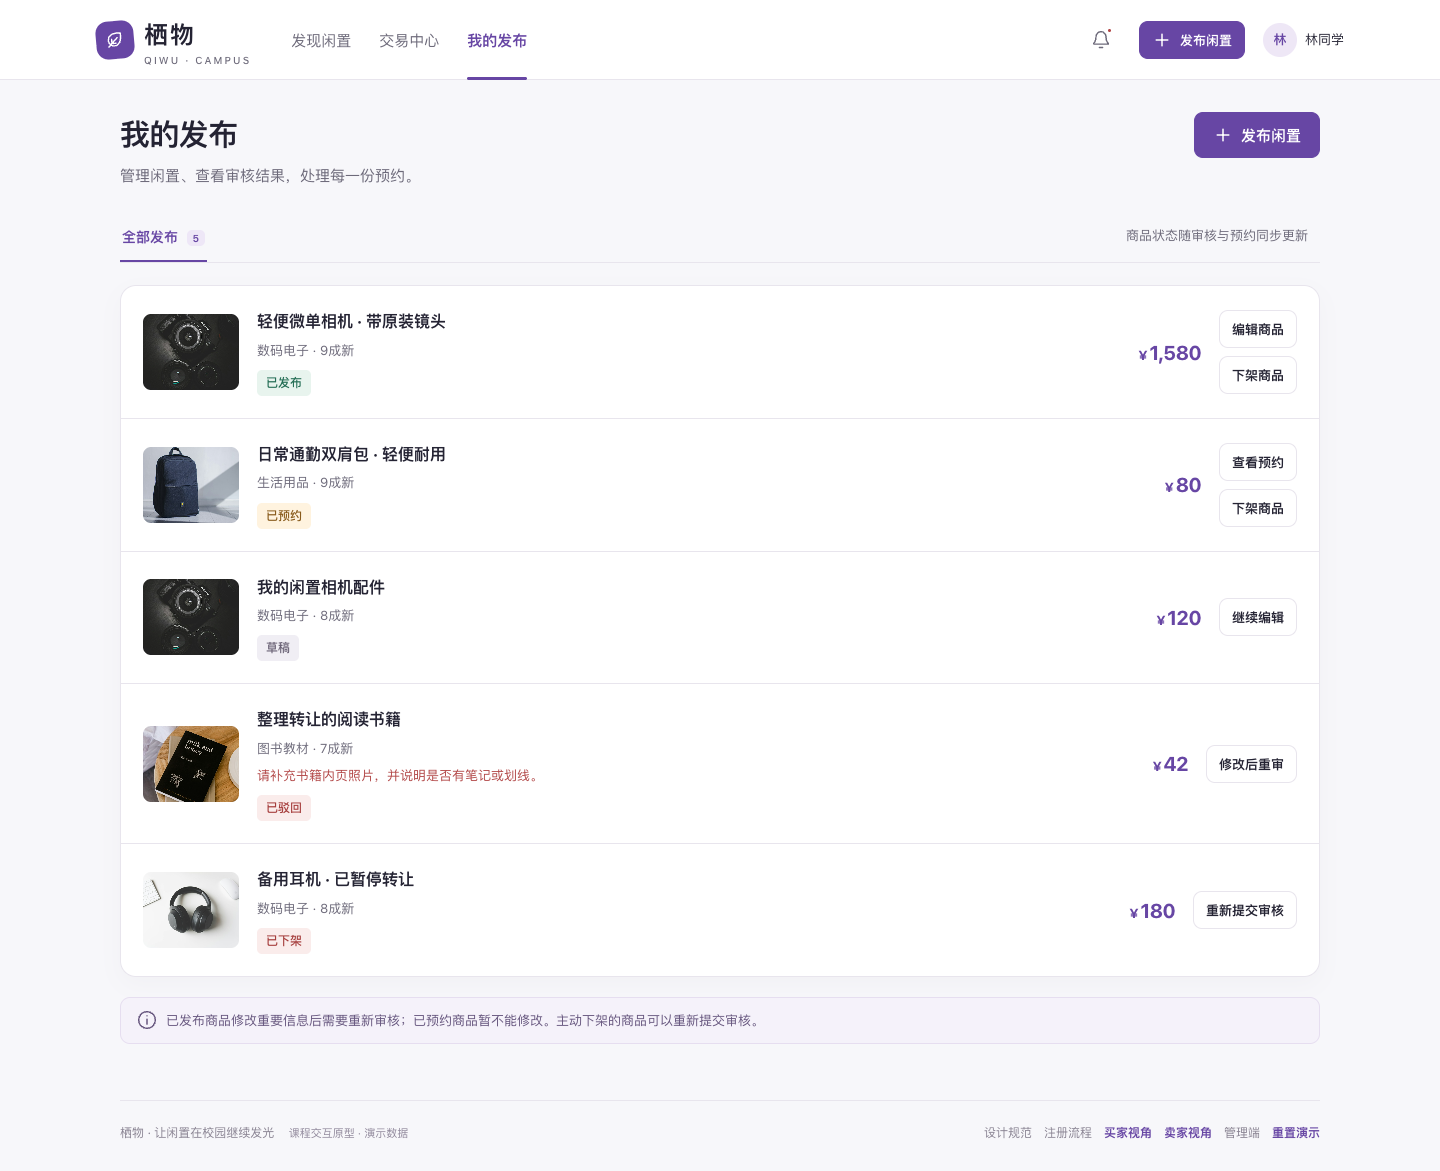
\includegraphics[width=\linewidth,height=91mm,keepaspectratio]{ui06.png}
    \caption{我的发布}
  \end{subfigure}
  \caption{商品编辑与状态管理}\label{fig:publish}
\end{figure}
\textbf{相关模块：}商品管理、审核。发布可以先保存草稿，正式提交再检查完整性；面交地点选填。我的发布根据状态提供编辑、重审、下架或查看预约入口，重要修改须重新审核。
\clearpage

\subsection{交易详情、记录与通知}
\reportfigure{ui04.png}{113mm}{交易详情与当前待办}{fig:trade}
\textbf{相关模块：}预约与交易、通知。交易页首先回答“目前是什么状态、下一步由谁操作”，再展示商品与历史。把最需要的信息放在前面，比单纯增加进度图标更有用。卖家接受后，双方可主动授权填写面交联系方式；预约终止时清除该字段。

\begin{figure}[H]\centering
  \begin{subfigure}[t]{0.48\linewidth}\centering
    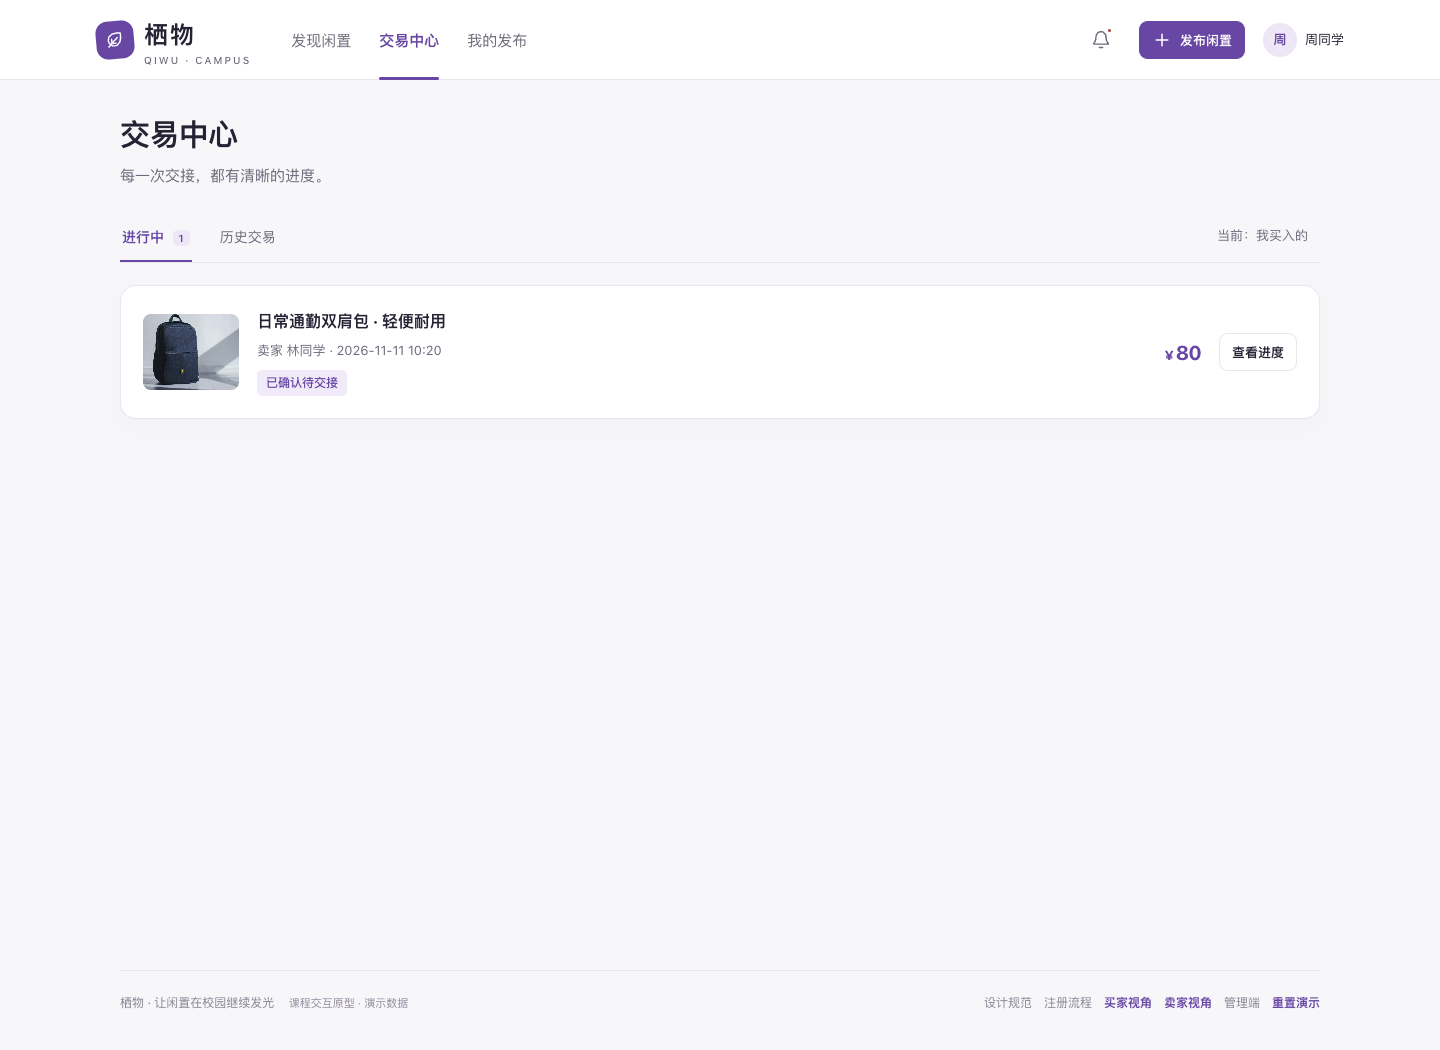
\includegraphics[width=\linewidth,height=63mm,keepaspectratio]{ui03.png}
    \caption{交易中心}
  \end{subfigure}\hfill
  \begin{subfigure}[t]{0.48\linewidth}\centering
    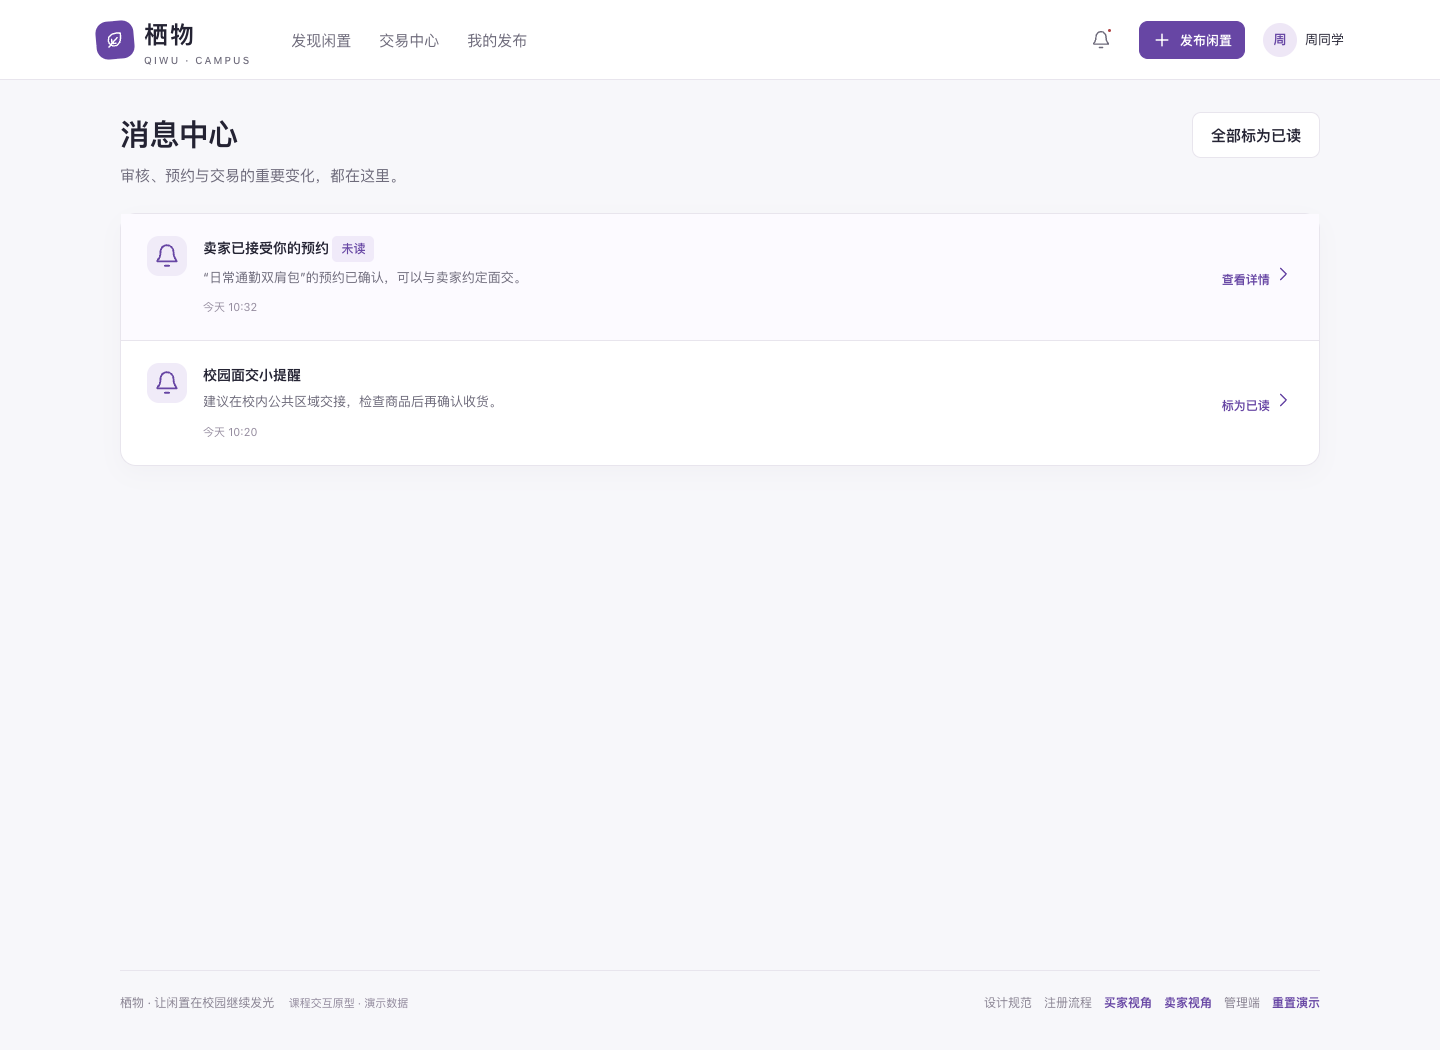
\includegraphics[width=\linewidth,height=63mm,keepaspectratio]{ui07.png}
    \caption{消息中心}
  \end{subfigure}
  \caption{交易记录与通知入口}\label{fig:notice}
\end{figure}
取消、下架等操作先说明影响，再要求确认。消息链接到对应的商品或预约，进入目标页面时仍需重新检查权限，不能因为收到了通知就跳过授权。
\clearpage

\subsection{管理概览与商品审核}
\reportfigure{ui10.png}{97mm}{管理概览}{fig:overview}
\textbf{相关模块：}统计与日志。展示商品总数、分类及状态分布、有效预约和已完成交易数量，统计口径为当前保存记录。待审核、驳回和已发布商品要分别计数。

\reportfigure{ui11.png}{97mm}{商品审核}{fig:review}
\textbf{相关模块：}审核与治理。队列和详情并排，减少反复切页。驳回必须说明原因，审核绑定商品版本，避免通过旧页面批准已经修改的内容。页面上的“通过”是一次业务操作，不只是改变颜色或标签。
\clearpage

\subsection{商品治理、账号与操作日志}
\begin{figure}[H]\centering
  \begin{subfigure}[t]{0.48\linewidth}\centering
    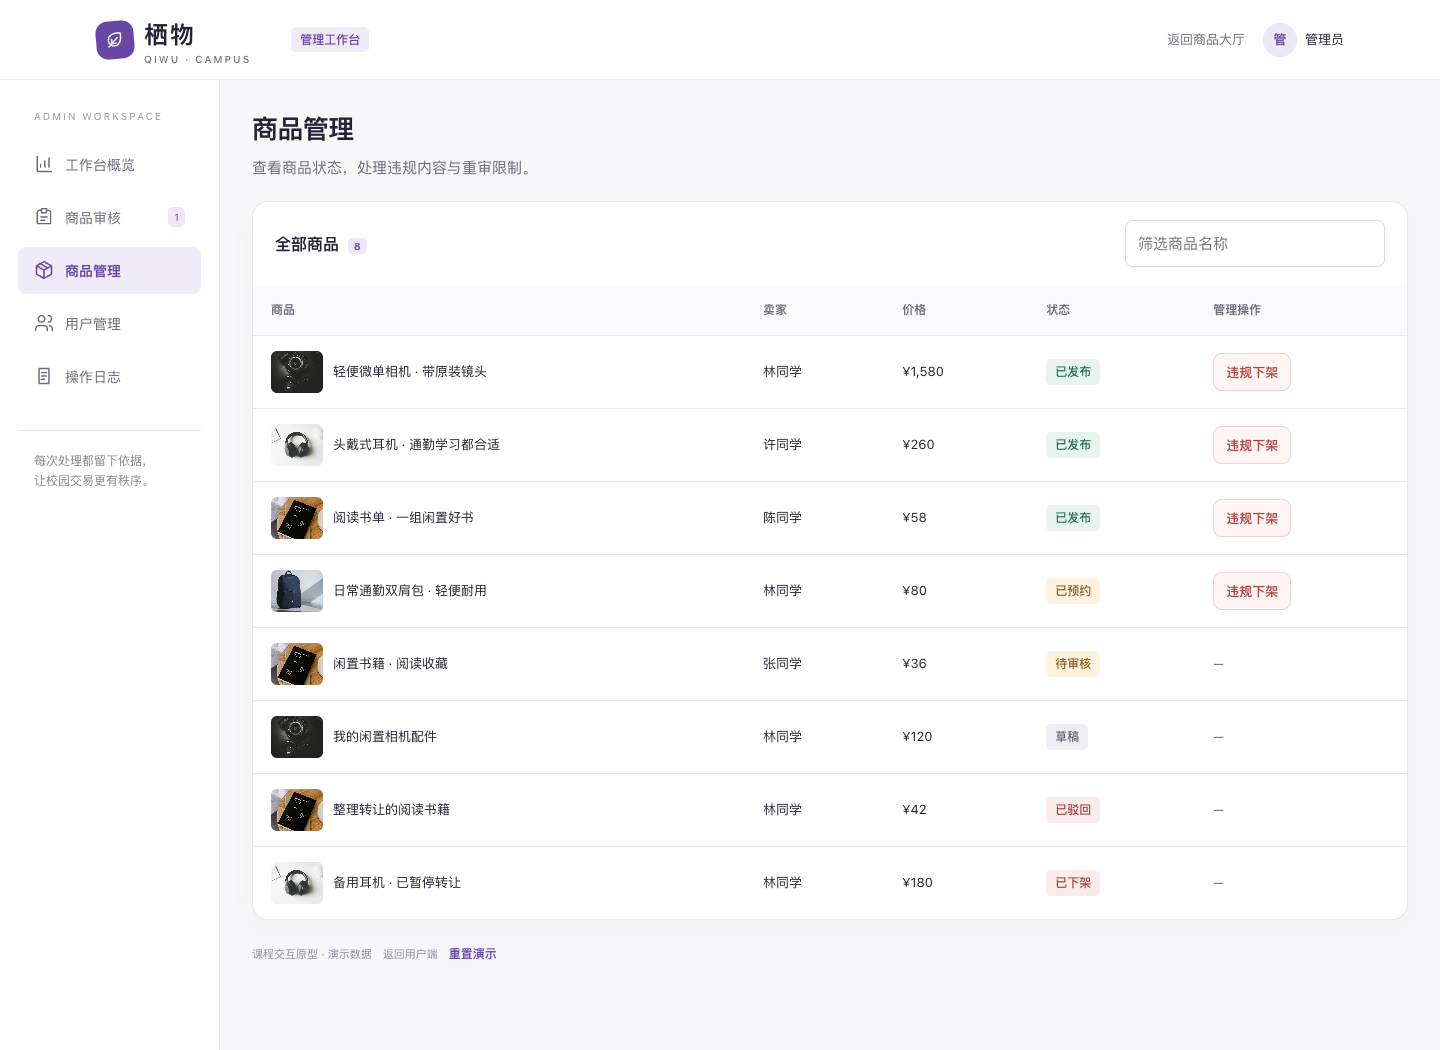
\includegraphics[width=\linewidth,height=74mm,keepaspectratio]{ui12.png}
    \caption{商品管理}
  \end{subfigure}\hfill
  \begin{subfigure}[t]{0.48\linewidth}\centering
    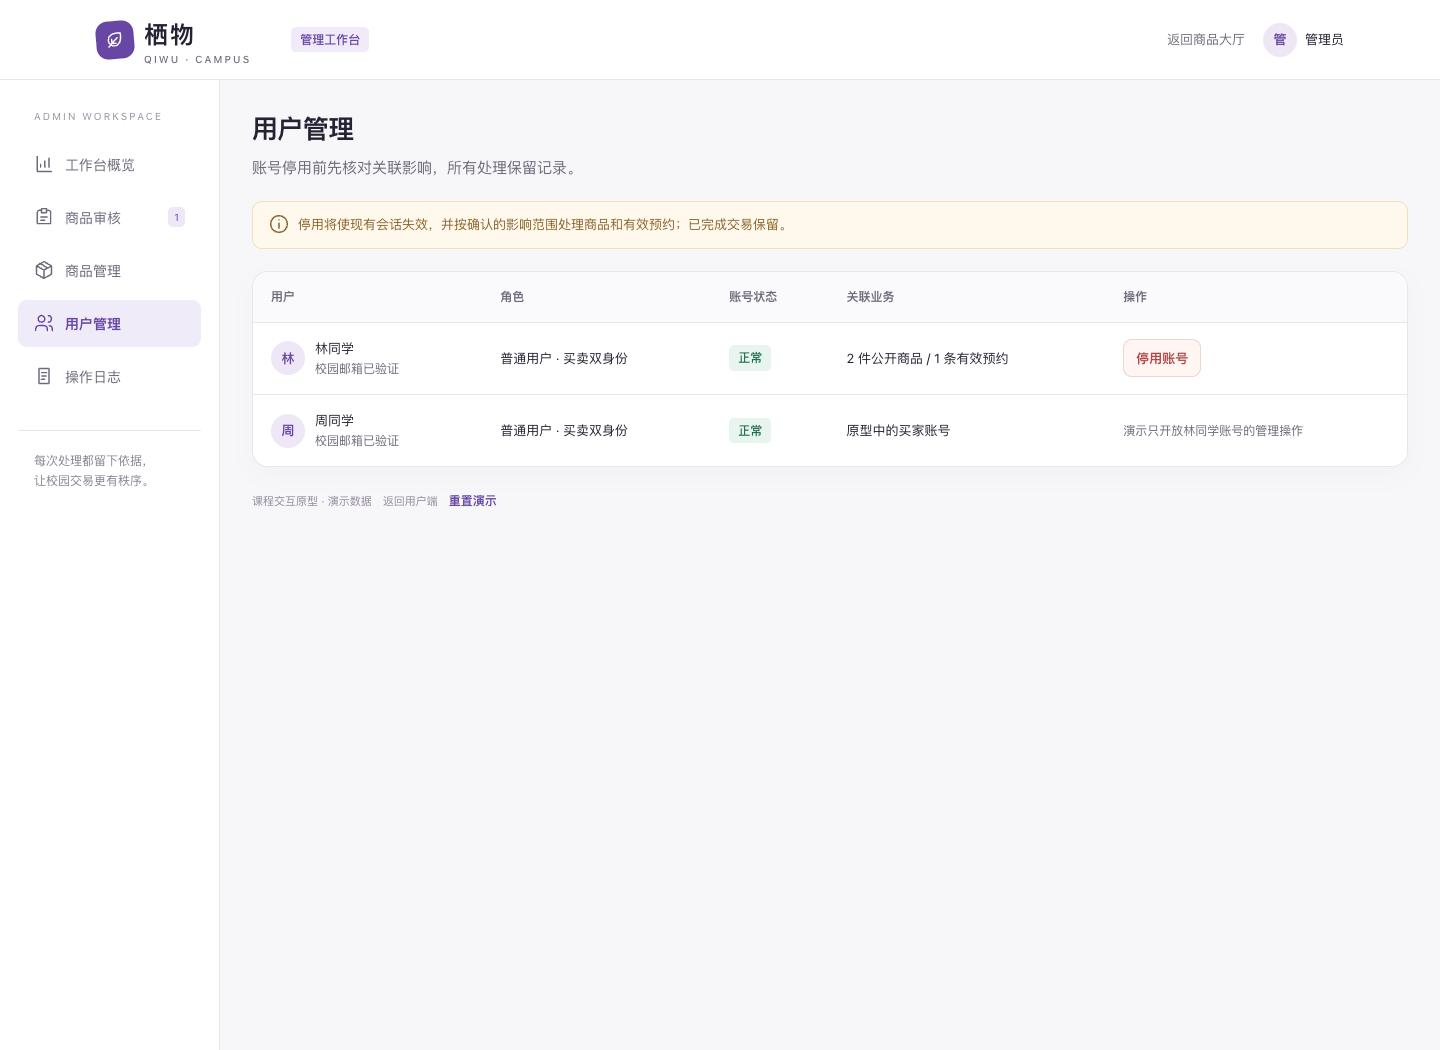
\includegraphics[width=\linewidth,height=74mm,keepaspectratio]{ui13.png}
    \caption{用户管理}
  \end{subfigure}
  \caption{违规处理与账号管理}\label{fig:governance}
\end{figure}
\textbf{相关模块：}审核与治理、账号与身份。违规下架和账号停用都可能影响现有预约，所以操作前显示影响范围并要求填写原因。恢复账号不自动恢复商品，解除重审限制也不直接发布，避免一次恢复操作带来意外的公开状态。

\reportfigure{ui14.png}{104mm}{操作日志}{fig:audit}
\textbf{相关模块：}统计与日志。记录操作者、时间、业务对象、动作和结果，只提供查询。失败的关键操作也要留痕，但密码、验证码和联系方式不进入日志。停用联动和联系字段清理属于本次设计补充，后续实现时仍需检查其实际效果。
\clearpage

\section{大模型的使用与思考}
\subsection{使用过程与修改}
本次使用Codex辅助整理需求、生成PlantUML与界面、检查交互和排版。UI先制作HTML/CSS原型，再导出draw.io可编辑稿；图源在本地渲染。各阶段的使用与取舍如下。

\begin{center}\small
\begin{tabularx}{\linewidth}{@{}p{14mm}*{3}{>{\raggedright\arraybackslash}X}@{}}\toprule
阶段 & 生成结果及优点 & 暴露的问题 & 修改与取舍 \\\midrule
规划 & 汇总需求，给出实现建议 & 建议仍需结合课程规模判断 & 结合课程规模与事务需求，采用单体方案 \\
设计 & 生成UML和页面，便于整体比较 & 存在样本状态、通知目标和联系入口遗漏 & 统一关键页风格与信息密度，补齐联系授权和通知目标 \\
检查 & 可重复运行交互检查 & 测试的身份重置也曾出错，初次图稿有截断 & 修正检查与导出脚本，重新渲染和验证 \\
报告 & 便于整理图号与说明 & 最初版本过长，说明重复 & 压缩重复说明，使用\LaTeX{}统一图题、目录与分页 \\\bottomrule
\end{tabularx}
\end{center}

设计取舍集中在实现成本、状态一致性和任务信息层次。AI生成结果经过问题检查与修正；权限、事务和性能方面尚未完成的验证另行列出。Git按领域模型、设计论证和报告记录本阶段成果，实验1基线保持不变。

\subsection{设计检查与尚未完成的部分}
已完成14项本地原型检查，包括预约到双确认、下架联动、超时边界、联系授权与清理；在1280px和390px下检查5类页面，未发现横向溢出。这只能说明演示交互可用。真实身份授权、邮件、持久化、并发竞争和故障回滚仍需实验3实现后测试。

\subsection{思考与总结}
本次设计中比较值得保留的有三点：接受预约与交易完成分开，避免把“愿意交易”误当成“已经交货”；主动下架与违规下架区别处理，在可用性与审核之间作取舍；交易页突出下一步操作，让用户知道当前该做什么。这些决定比页面数量更能体现设计是否贴合实际使用。

AI适合生成初稿和执行重复检查，但不能根据截图好看就判断业务正确。可行的流程是先明确需求和约束，再生成候选方案，由人判断关键取舍，最后用具体流程和异常情况验证。人的工作可以集中在检查与决策，却不能省掉对规则本身的理解。

\vspace{1mm}
\noindent\textbf{参考资料}\quad
本课程实验手册及实验1需求；\href{https://plantuml.com/}{PlantUML官方文档}；\href{https://docs.djangoproject.com/en/5.2/ref/databases/}{Django数据库说明}。UI示意照片来自Unsplash；原始链接与图稿对应表见源文件包中的说明文件。

\end{document}
